\documentclass[11pt]{article}
\usepackage{amsmath}
\usepackage{geometry}                % See geometry.pdf to learn the layout options. There are lots.
\geometry{letterpaper}                   % ... or a4paper or a5paper or ... 
%\geometry{landscape}                % Activate for for rotated page geometry
%\usepackage[parfill]{parskip}    % Activate to begin paragraphs with an empty line rather than an indent
\usepackage{graphicx}
\usepackage{fullpage}
\usepackage{amssymb}
\usepackage{epstopdf}
\usepackage{url}
\DeclareGraphicsRule{.tif}{png}{.png}{`convert #1 `dirname #1`/`basename #1 .tif`.png}
\date{}
\title{Homework 2}
\author{(Inference and Representation) 
\\ Due October 2 on NYU Classes.  }
%\date{}                                           % Activate to display a given date or no date

\begin{document}
\maketitle
 
\begin{enumerate}
\item Consider the Bayesian Network below:

\begin{center}
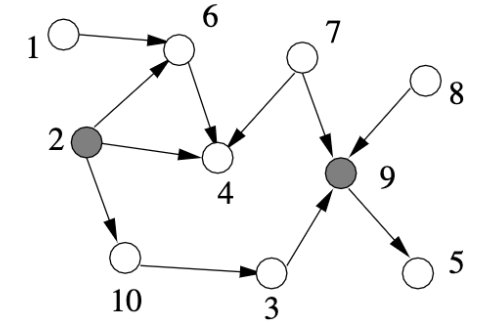
\includegraphics[width=.3\textwidth]{graph}
\end{center}
\begin{enumerate}
\item For what pairs $(i,j)$ does the statement $X_i \perp X_j$ hold? (Do not assume any conditioning for this part).
\item Suppose that we condition on $\{X_2, X_9\}$, shown shaded in the graph. What is the largest set $A$ for which the statement $X_1 \perp X_A | \{X_2, X_9\}$ holds? 
\end{enumerate}

\item Consider the following distribution over 3 binary variables $X,Y,Z:$
$$
\operatorname{Pr}(x,y,z)=\left\{ 
\begin{matrix}
1/12 & x \oplus y \oplus z =0 \\
1/6 & x \oplus y \oplus z =1 
\end{matrix}
\right.
$$
where $\oplus$ denotes the XOR function. Show that there is no directed acyclic graph $G$ such that $I_{d-sep}(G)= I(Pr)$.


\item The Ising model, from statistical physics, consists of discrete variables that represent magnetic spins that can be in one of two states (+1 or -1). The spins are arranged in a graph, usually a lattice, allowing each spin to interact with its neighbors. It satisfies the distribution
\begin{equation} \label{ising}
\operatorname{Pr}(x_1,\ldots, x_n)= \frac{1}{Z} \exp\left(\sum_{(i,j)\in E} w_{i,j}x_i x_j - \sum_{i\in V} u_i x_i \right),
\end{equation}
where the random variables $X_{i}\in \{+1, -1\}$. Related to the Ising model is the Boltzmann machine, which is an early model for neural networks. Boltzmann machines are parameterized the same way (i.e., using \eqref{ising}), but it has variables $X_i \in\{ 0, 1\}$. Here we get a non-zero contribution to the energy (i.e. the quantity in the parentheses in \eqref{ising}) from an edge $(i, j)$ only when $X_i = X_j = 1$.
Show that a Boltzmann machine distribution can be rewritten as an Ising model. More specifically, given parameters $\mathbf w, \mathbf u$ corresponding to a Boltzmann machine, specify new parameters $\mathbf{w'}, \mathbf {u'}$ for an Ising model and prove that they give the same distribution Pr$(X)$ (assuming the state space $\{0, 1\}$ is mapped to $\{-1, +1\}$).

\item Let $T$ denote the edges of a tree-structured pairwise Markov random field with vertices $V$ . For the special case of trees, prove that any distribution $p_T(x)$ corresponding to a Markov random field over $T$ admits a factorization of the form:
$$p_T(x)=\Pi_{(i,j)\in T} \frac{p_T(x_i,x_j)}{p_T(x_i)p_T(x_j)} \Pi_{j\in V} p_T(x_j), $$
where $p_T(x_i,x_j)$ and $p_T(x_i)$ denote pairwise and singleton marginals of the distribution $p_T$ , respectively.

Hint: consider the Bayesian network where you choose an arbitrary node to be a root and direct all edges away from the root. Show that this is equivalent to the MRF. Then, looking at the BN’s factorization, reshape it into the required form.

\item Recall the occasionally dishonest casino example we saw in class (from Durbin et al. 1998, see chapter 17 of Murphy). A casino has two dice, one is fair (every number in $\{1,2,3,4,5,6\}$ is cast with the same probability) and the other one is loaded but we don't know the exact distribution of its outputs. The casino starts using a fair die but with some unknown probability it switches to the loaded die back and forth. The goal of this problem is to learn the HMM model from the dataset \texttt{sequence.txt}. In particular the transition probabilities between the hidden states (loaded to fair and fair to loaded) and the probability distribution of the output of the loaded dice.  

Someone suggested that the casino had actually three different dice, one fair and two loaded with different probabilities. How would the Hidden Markov Model look in this case? Which one do you think is more likely?

Hint: The Baum-Welch algorithm may be useful. If you use a software package you need to explain what it's doing.

\end{enumerate}
\end{document}  